% copyrights 2009 Dave Liu

%\documentclass[12pt]{beamer}
\documentclass[handout]{beamer}

\usepackage{amsmath}
\usepackage{amssymb} % http://www.ctan.org/tex-archive/macros/latex/required/psnfss/psnfss2e.pdf
\usepackage{helvet}

\usecolortheme{dolphin}
\useoutertheme{infolines}



\title [Money in Flexible Price Environments: CIA]{Money in Flexible Price Environments: CIA}
\vskip 0.1in

\subtitle{Dynamic Economic Theory (871)}
\author[H Hollander]{Hylton Hollander}

\institute[University of Stellenbosch]{\large{Department of Economics\\
University of Stellenbosch}}


\date[March 19, 2015]{March 19, 2015}

\begin{document}

\frame{\titlepage}

\frame{\frametitle{Contents:} \tableofcontents}


\begin{frame}

\frametitle{Readings} \vskip 0.1in


\begin{itemize}
\item Walsh, C. E., 2010. Monetary Theory and Policy, 3rd Ed. The MIT Press. (CH 3) \\
\vskip 0.1in
\item Cooley, T. F. and G. D. Hansen, 1989. The inflation tax in a
real business cycle model. \emph{American Economic Review}, 79:
733-748.
\end{itemize}
\end{frame}


\section{Introduction}

\begin{frame}
\frametitle{Introduction} \vskip 0.1in
%reference: Walsh: 43

\begin{itemize}
\item The Neoclassical growth model is a model of nonmonetary
economy, in which goods are exchanged and transactions must be
taking place. In the economy, there is neither medium of exchange
(money) that is used to facilitate these transactions, nor an asset
like money that has a zero nominal return and is therefore dominated
in rate of return by other interest-bearing assets.

\item In order to study monetary issues using the Neoclassical
framework, we need to introduce money into the model economy and
motivate agents to hold positive quantity of money

\item There are different approaches to introducing money into the
Neoclassical growth model. We will study the most popular two, the
cash in advance (CIA) model and money in utility (MIU) model.
\end{itemize}


\end{frame}

\begin{frame}
\frametitle{Introduction} \vskip 0.1in
%reference: Walsh: 43

\begin{itemize}
\item The MIU model (Sidrauski, 1967) assumes that money itself yield direct utility
by incorporating real money balances in the utility functions of the
agents of the model, whereas in the CIA model, money is a medium of
exchange for purchasing consumption goods. \vskip 0.2in

\item In this session, we will look at the CIA model due to Clower
(1967) and Lucas (1982). The model described here is the
Cooley-Hansen(1989) CIA model.
\end{itemize}
\end{frame}

\section{The Model}

\begin{frame}
\frametitle{The Model} \vskip 0.1in
%reference:

\textcolor{green}{Firm}\vskip 0.1in

Aggregate output is produced according to the following constant
returns to scale technology:

\begin{equation}\label{Eq4.1}
y_{t}=f(k_{t-1},n_{t},z_{t})=e^{z_{t}}k_{t-1}^{\alpha}n_{t}^{1-\alpha}
\end{equation}

where the technology shock $z_{t}$ follows:
\begin{equation}\label{Eq4.2}
z_{t}=\rho_{z} z_{t-1} + \epsilon_{z,t}, ~ \qquad 0<\rho_{z}<1, ~
\qquad \epsilon_{z,t} \sim i.i.d.(0,\sigma_{z}^{2})
\end{equation}

and the capital accumulation equation:
\begin{equation}\label{Eq4.3}
k_{t}=(1-\delta)k_{t-1}+x_{t}
\end{equation}
\end{frame}


\begin{frame}
\frametitle{The Model} \vskip 0.1in
%reference:

\textcolor{green}{Household}\vskip 0.1in

Household maximizes the discounted expected utility function:
\begin{equation}\label{Eq4.4}
E_{0}\sum_{t=0}^{\infty} \beta^{t} U(c_{t}, 1-n_{t}) =
E_{0}\sum_{t=0}^{\infty} \beta^{t}
[\frac{c_{t}^{1-\eta_{c}}}{1-\eta_{c}} +
\frac{(1-n_{t})^{1-\eta_{n}}}{1-\eta_{n}}]
\end{equation}
\pause
s.t.\\
the budget constraint:
\begin{equation}\label{Eq4.5}
y_{t}+\tau_{t}+(1-\delta)k_{t-1}+\frac{m_{t-1}}{1+\pi_{t}} +
\frac{b_{t-1}(1+i_{t-1})}{1+\pi_{t}} \geq c_{t}+k_{t}+m_{t} + b_{t}
\end{equation}
\pause and the CIA constraint:
\begin{equation}\label{Eq4.6}
C_{t} \leq M_{t-1}+ T_{t} - B_{t}, ~~or~~ c_{t}\leq
\frac{m_{t-1}}{1+\pi_{t}}+\tau_{t} - b_{t} ~~(in ~real ~term)
\end{equation}
\end{frame}



\begin{frame}
\frametitle{The Model} \vskip 0.1in

\textcolor{green}{Government budget constraint}

\begin{equation}\label{Eq4.7}
T_{t}=\bar{M}_{t} - \bar{M}_{t-1}
\end{equation}

\textcolor{green}{Money creation process}
\begin{itemize}
\item Money growth
\begin{equation}\label{Eq4.8}
\bar{M}_{t}=(1+\theta_{t})\bar{M}_{t-1}
\end{equation}

\pause

\item Money supply shock
\begin{equation}\label{Eq4.9}
\mu_{t}=\rho_{m}\mu_{t-1} + \phi z_{t-1} +\epsilon_{m,t} \qquad
\rho_{m}>0, \qquad \epsilon_{m,t} \sim i.i.d.(0,\sigma_{m}^{2})
\end{equation}
where
\begin{equation}\label{Eq4.10}
\mu_{t}=\theta_{t}-\bar{\theta}
\end{equation}

\end{itemize}


\end{frame}

\begin{frame}
\frametitle{The Model} \vskip 0.1in

\textcolor{blue}{Remarks}

\begin{itemize}
\item Timing: The timing is that assets market opens first (Lucas,
1982). Agents only hold an amount of money that is just sufficient
to finance their desired level of consumption at the beginning of
each period, \emph{after observing any current shocks}. In other
words, household is able to adjust its portfolio between money and
other assets (bonds) before entering the goods market (Walsh: 101).

\item In the case of goods market opens first (Svensson, 1985), households enter time
period t with money holding $m_{t-1}$ and receives a lump-sum
transfer $\tau_{t}$. Households cannot adjust their portfolio after
shocks hit\footnote{Since we focus on the impact of money, without loss of generality, we exclude bonds in the model.}.


\item Since the opportunity cost of holding money
is positive as long as the nominal interest rate is greater than
zero, $\rho_{m}$ should always be greater than zero. The CIA
constraint \eqref{Eq4.6} is always binding.


\end{itemize}




\end{frame}



\section{Solving the Model}

\begin{frame}
\frametitle{Solving the Model} \vskip 0.1in

Household's decision is characterized by the following value
function:

\begin{equation}\label{Eq4.11}
V(k_{t-1}, m_{t-1}, z_t, \mu_t)= \max_{c_{t},n_{t},k_{t},m_{t}}
[U(c_{t},1-n_{t})+\beta E_{t}V(k_t, m_{t})]
\end{equation}

where
\begin{equation}\tag{\eqref{Eq4.4}}
   U(c_{t},1-n_{t})=\frac{c_{t}^{1-\eta_{c}}}{1-\eta_{c}}+\frac{(1-n_{t})^{1-\eta_{n}}}{1-\eta_{n}}
\end{equation}

\pause

Following Walsh
(2003)\footnote{$y_{t}=f(k_{t-1},n_{t},z_{t})=z_{t}k_{t-1}^{\alpha}n_{t}^{1-\alpha}$}:
\begin{itemize}
\item define $\omega_{t}=y_{t}+(1-\delta)k_{t-1}+\tau_{t}+\frac{m_{t-1}}{1+\pi_{t}}$
\item define $\lambda_{t}$ and $\Lambda_{t}$ are the multipliers of
budget constraint and CIA constraint respectively
\end{itemize}
\end{frame}

\begin{frame}
\frametitle{Solving the Model} \vskip 0.1in

\textcolor{blue}{FOCs w.r.t. \{$c_{t},n_{t},k_{t},m_{t}$\}:}
\begin{eqnarray}
\lambda_{t} + \Lambda_{t} &=& U_{c}(c_{t}, 1-n_t) \label{Eq4.12}\\
(1-\alpha)z_{t}k_{t-1}^{\alpha}n_{t}^{-\alpha}\lambda_{t} &=&
U_{n}(c_{t}, 1-n_t)  ~~\label{Eq4.13}\\
\beta R_{t}E_{t} V_{k}(k_t,m_{t})&=& \lambda_{t} \label{Eq4.14}\\
\beta E_{t} [\frac{\lambda_{t+1}+\Lambda_{t+1}}{1+\pi_{t+1}}] &=&
\lambda_{t}\label{Eq4.15}
\end{eqnarray}
\end{frame}


\begin{frame}
\frametitle{Solving the Model}
\vskip 0.1in

\textcolor{blue}{Remarks}\vskip 0.1in

$\square$ Recall \eqref{Eq4.12}:
\begin{equation}\tag{\eqref{Eq4.12}}
\lambda_{t} + \Lambda_{t} = U_{c}(c_{t}, 1-n_t)
\end{equation}

$MU_{c}$ is the sum of the $MU_{\omega}$, $\lambda_{t}$, and the
value of the liquidity service (cost of holding money),
$\Lambda_{t}$, needed to finance the transaction.

\vskip 0.1in \pause

$\square$ Substitute $\lambda_{t+1} = V_{k}(k_t,m_{t})$ into
\eqref{Eq4.14}:

\begin{equation}\label{Eq4.16}
\beta R_{t}E_{t}\lambda_{t+1} = \lambda_{t}
\end{equation}

\eqref{Eq4.16} is the standard asset pricing equation. The MC from
reducing wealth today, $\lambda_{t}$, must equal to the utility
value of carrying that wealth forward one period, earning a gross
real rate of return $R_{t}$, where tomorrow's utility is discounted
back to today at rate $\beta$ (Walsh 2003: 105).

\end{frame}

\begin{frame}
\frametitle{Solving the Model} \vskip 0.1in

\textcolor{blue}{Remarks}\vskip 0.1in

$\square$ Recall \eqref{Eq4.15}:

\begin{equation}\tag{\eqref{Eq4.15}}
\beta E_{t} [\frac{\lambda_{t+1}+\Lambda_{t+1}}{1+\pi_{t+1}}] =
\lambda_{t}
\end{equation}

\begin{eqnarray}
\beta E_{t} [\frac{\lambda_{t+1}+\Lambda_{t+1}}{P_{t+1}/P_{t}}] &=&
\lambda_{t}\label{Eq4.17}\\
\beta E_{t} [\frac{\lambda_{t+1}+\Lambda_{t+1}}{P_{t+1}\lambda_{t}}]
&=& \frac{1}{P_{t}}\label{Eq4.18}
\end{eqnarray}

\eqref{Eq4.18} is the asset pricing equation for money. The
price/value of a unit of money in terms of goods, $\frac{1}{P_{t}}$,
is equal to discounted marginal benefit from future earnings (value
of money).

\end{frame}


\section{Why Inflation Tax?}
%ref: Walsh 2003: 106-107

\begin{frame}
\frametitle{Why Inflation Tax?}\vskip 0.1in

In Cooley-Hansen CIA model, a positive nominal interest rate acts as
a tax on consumption. Why?\\\vskip 0.1in

Combining \eqref{Eq4.15} and \eqref{Eq4.16}, we have:

\begin{equation}\label{Eq4.37}
\beta E_{t} [\frac{\lambda_{t+1}+\Lambda_{t+1}}{1+\pi_{t+1}}] =
\beta R_{t}E_{t}\lambda_{t+1}
\end{equation}

or

\begin{equation}\label{Eq4.38}
E_{t} [\lambda_{t+1}+\Lambda_{t+1}] =
R_{t}E_{t}[\lambda_{t+1}(1+\pi_{t+1})]
\end{equation}

Since $1+i_{t} = R_{t}(1+\pi_{t+1})$, \eqref{Eq4.37}
becomes\footnote{expectation is dropped here.}:

\begin{equation}\label{Eq4.39}
1+i_{t} = (\frac{\lambda_{t+1}+\Lambda_{t+1}}{\lambda_{t+1}})
\end{equation}


\end{frame}

\begin{frame}
\frametitle{Why Inflation Tax?}\vskip 0.1in

\begin{eqnarray}
i_{t} &=& (\frac{\lambda_{t+1}+\Lambda_{t+1}}{\lambda_{t+1}})-1
\label{Eq4.40}\\
i_{t} &=& \frac{\Lambda_{t+1}}{\lambda_{t+1}} \label{Eq4.41}
\end{eqnarray}

That is, if the CIA constraint is binding, then money has value
because it yields valued liquidity services. In this case, the
nominal interest rate is positive and it acts as a tax on
consumption.\\\vskip 0.1in

Inflation represents a tax on the purchases of the cash goods, and
therefore higher rate of inflation shifts household demand away from
cash good (consumption) and toward the credit good (such as leisure
and investment).

\end{frame}

\section{Steady States}

\begin{frame}
\frametitle{Steady States}\vskip 0.1in

\begin{eqnarray}
R^{ss} &=& \frac{1}{\beta} \label{Eq4.19}\\
\frac{y^{ss}}{k^{ss}} &=& \frac{1}{\alpha}(R^{ss}
-1+\delta)\label{Eq4.20}\\
\frac{c^{ss}}{k^{ss}} &=& \frac{y^{ss}}{k^{ss}}-\delta
\label{Eq4.21}\\
\frac{n^{ss}}{k^{ss}} &=&
(\frac{y^{ss}}{k^{ss}})^{\frac{1}{1-\alpha}} \label{Eq4.22}\\
\frac{(n^{ss})^{\eta_{c}}}{(1-n^{ss})^{\eta_{n}}} &=& (1-\alpha)
\frac{\beta}{1+\pi^{ss}} (\frac{c^{ss}}{k^{ss}})^{-\eta_{c}}
(\frac{y^{ss}}{k^{ss}})^{\frac{\eta_{c}-\alpha}{1-\alpha}}
\label{Eq4.23}
\end{eqnarray}

\end{frame}


\begin{frame}
\frametitle{Steady States}\vskip 0.1in

$\square$ Welfare cost of inflation in CIA model (Cooley-Hansen model) \\
\vskip 0.1in

In steady state, the binding CIA constraint gives:

\begin{equation}\label{Eq4.24}
c^{ss}=\frac{m^{ss}}{1+\pi^{ss}}+\tau^{ss}=m^{ss}
\end{equation}

Therefore:
\begin{equation}\label{Eq4.25}
\frac{c^{ss}}{k^{ss}}=\frac{m^{ss}}{k^{ss}}
\end{equation}

Recall \eqref{Eq4.23}:

\begin{equation}\tag{\eqref{Eq4.23}}
(1-n^{ss})^{-\eta_{n}} (n^{ss})^{\eta_{c}} = (1-\alpha)
\frac{\beta}{1+\pi^{ss}} (\frac{c^{ss}}{k^{ss}})^{-\eta_{c}}
(\frac{y^{ss}}{k^{ss}})^{\frac{\eta_{c}-\alpha}{1-\alpha}}
\end{equation}

$\Rightarrow$ $n^{ss}\downarrow$ if $\theta^{ss}\uparrow$ (with the
CIA constraint binding, in steady state $\pi^{ss}=\theta^{ss}$)


\end{frame}


\begin{frame}
\frametitle{Steady States}

$\square$ The superneutrality of money \\

\begin{itemize}
\item The model exhibits the neutrality property: proportional
changes in the level of nominal money balances and prices do not affect real
variables.
\item In \eqref{Eq4.19} $\backsim$ \eqref{Eq4.22}, none of the steady
state values/ratios depend on the growth rate of nominal money
supply --- CIA model exhibits superneutrality iff labor supply is
inelastic\footnote{As shown in \eqref{Eq4.23}, labor supply is
affected by money supply!}, that is, $n\equiv1$.
\end{itemize}
\pause

$\square$ The optimal rate of inflation \\

An efficient equilibrium will be characterized by
equality between social and private costs. Because the social cost
of producing money is zero, the private opportunity cost of holding
money must be zero in order to achieve optimality.\\\vskip 0.05in

The private opportunity cost is measured by the nominal interest
rate, so the optimal rate of inflation in the steady state is the
rate that achieves a zero nominal rate of interest --- deflation
(Walsh 2003: 126).

\end{frame}







\section{Dynamics}

\begin{frame}
\frametitle{Dynamics}\vskip 0.1in

The linearized model:\\

{\scriptsize{
\begin{eqnarray}
\hat{y}_{t} &=& \alpha \hat{k}_{t-1}+(1-\alpha)\hat{n}_{t}+z_{t}\label{Eq4.26}\\
(\frac{y^{ss}}{k^{ss}})\hat{y}_{t} &=&
(\frac{c^{ss}}{k^{ss}})\hat{m}_{t} +
\hat{k}_{t} -(1-\delta)\hat{k}_{t-1}\label{Eq4.27}\\
\hat{r}_{t} &=& \alpha (\frac{y^{ss}}{k^{ss}})
(E_{t}\hat{y}_{t+1}-\hat{k}_{t})\label{Eq4.28}\\
\hat{\lambda}_{t} &=& E_{t} \hat{\lambda}_{t+1} + \hat{r}_{t}\label{Eq4.29}\\
\hat{y}_{t} + \hat{\lambda}_{t} &=&
(1+\eta_{n}\frac{n^{ss}}{1-n^{ss}})\hat{n}_{t}\label{Eq4.30}\\
\hat{i}_{t} &=& \hat{r}_{t} + E_{t}\hat{\pi}_{t+1}\label{Eq4.31}\\
\hat{\lambda}_{t} &=& -E_{t} (\eta_{c} \hat{m}_{t+1} +
\hat{\pi}_{t+1})\label{Eq4.32}\\
\hat{m}_{t} &=& \hat{m}_{t-1} - \hat{\pi}_{t} +
\mu_{t}\label{Eq4.33}
\end{eqnarray}

To complete the model, we add the disturbances:

\begin{eqnarray}
\hat{z}_{t} &=& \rho_{z} \hat{z}_{t-1}+\epsilon_{z,t} \label{Eq4.34}\\
\hat{\mu}_{t} &=& \rho_{m}\hat{\mu}_{t-1}+\phi
\hat{z}_{t-1}+\epsilon_{m,t} ~ , ~~~ \phi = 0 \label{Eq4.35}
\end{eqnarray}
}}

\end{frame}



\begin{frame}
\frametitle{Dynamics}\vskip 0.1in

$\square$ Updating \eqref{Eq4.33} one period ahead and substituting
into \eqref{Eq4.32}, and combining \eqref{Eq4.30}, we have:

\begin{equation}\label{Eq4.36}
\hat{y}_{t} = (1+\eta_{n}\frac{n^{ss}}{1-n^{ss}})\hat{n}_{t} +
(\hat{m}_{t}+E_{t}\mu_{t+1})
\end{equation}

It implies that given output, a positive shock in money supply in
\emph{t} will result a higher expected money growth in \emph{$t+1$},
and therefore higher expected inflation. This, in turn, results in a
fall in labor supply.\\\vskip 0.1in

\pause

$\square$ Now, let's now look at the impulse responses of the model
in respect to both the real shock and nominal shock.


\end{frame}

\begin{frame}

\frametitle{Dynamics (Impulse responses to a shock in
technology)}\vskip 0.1in

%ref: McCandless (2008): 210-211.

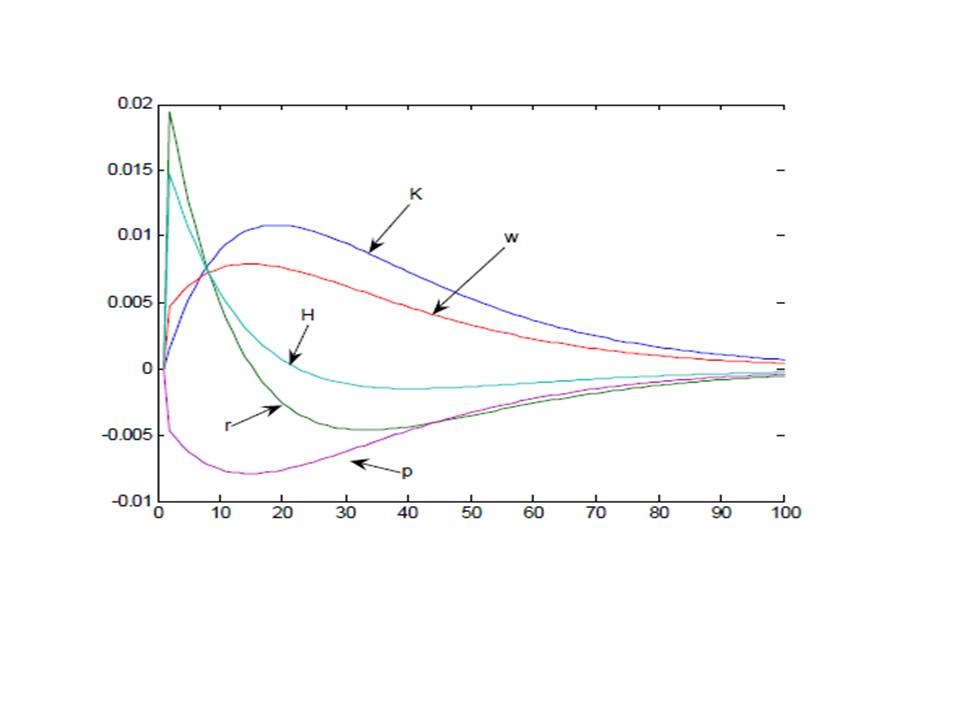
\includegraphics[width = 5.0in]{CIA_tech.jpg}

\end{frame}

\begin{frame}

\frametitle{Dynamics (Impulse responses to a shock in money)}\vskip
0.1in

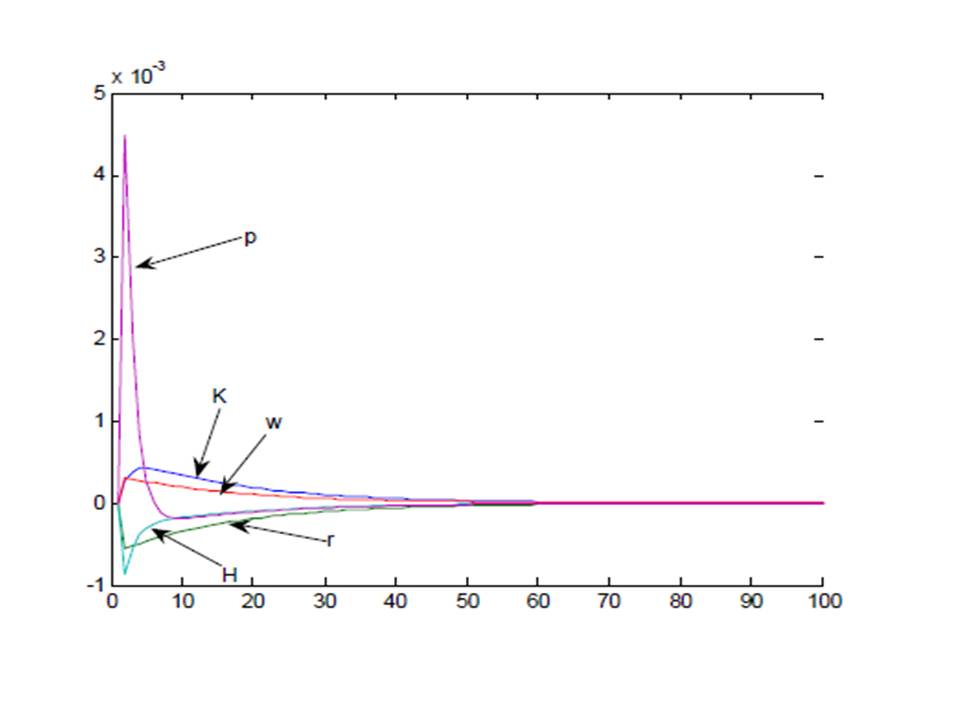
\includegraphics[width = 4.0in]{CIA_money.jpg}

\end{frame}


%\begin{comment}
%``Put differently, the nominal interest rate is the ratio between the expected marginal
%utility of the direct return on money and the expected utility of the indirect return
%on money. We can understand this relation as follows: money and bonds have the same
%indirect return. For one unit of money held as cash at the end of period t and one unit
%of money invested in a nominal bond at the end of period t, both ''pay'' one unit of
%money at the end of period t + 1 as indirect return. The expected utility of that indirect
%return is $\beta E(P_{t}\lambda_{t+1})$. In equilibrium, the expected utility of the liquidity services of one
%unit of money must equal the expected utility of the interest on one unit of money
%invested as a nominal bond. This gives rise to (12).'' ~~~ Lars Svensson, 1985, p.927
%\end{comment}


\begin{frame}
\begin{center}
\Huge{THE END}
\end{center}
\end{frame}

\appendix

\renewcommand{\theequation}{A.\arabic{equation}}
\setcounter{equation}{0}

\section{Appendix A: First Order Conditions}
\begin{frame}
\frametitle{Appendix A: First Order Conditions} \vskip 0.1in

Value function:
\begin{eqnarray}\label{Eq4a.1}
V(k_{t-1}, b_{t-1}, m_{t-1}, z_{t}, \mu_{t})&=& \max
[u(\frac{c_{t}^{1-\eta_{c}}}{1-\eta_{c}}+\frac{(1-n_{t})^{1-\eta_{n}}}{1-\eta_{n}})
+\beta E_{t}V(k_{t}, m_{t}) \nonumber\\ & &  +
\lambda_{t}(\omega_{t}- c_{t}-m_{t}-k_{t})  \nonumber\\ & & +
\Lambda_{t}(\frac{m_{t-1}}{1+\pi_{t}}+\tau_{t}-c_{t})]
\end{eqnarray}

where the maximization is with respect to
$\{c_{t},n_{t},k_{t},m_{t}\}$.

\vskip 0.1in \pause

\textcolor{blue}{FOCs:}

\begin{itemize}
\item $c_{t}$
\begin{eqnarray}
\frac{\partial V(k_{t-1}, b_{t-1},m_{t-1})}{\partial c_{t}} &=&
c^{-\eta_{c}}-\lambda_{t}-\Lambda_{t}\label{Eq4a.2}\\
\lambda_{t}+\Lambda_{t} &=& c^{-\eta_{c}}\label{Eq4a.3}
\end{eqnarray}
\end{itemize}
\end{frame}

\begin{frame}
\frametitle{Appendix A: First Order Conditions} \vskip 0.1in
\textcolor{blue}{FOCs:}

\begin{itemize}
\item $n_{t}\footnote{$k_{t-1}=f(k_{t-1},n_{t},z_{t})+(1-\delta)k_{t-1}+\tau_{t}+\frac{m_{t-1}}{1+\pi_{t}}$,
where
$f(k_{t-1},n_{t},z_{t})=z_{t}k_{t-1}^{\alpha}n_{t}^{1-\alpha}$}$
\begin{eqnarray}
\frac{\partial V(k_{t-1}, b_{t-1}, m_{t-1}, z_{t},
\mu_{t})}{\partial n_{t}} &=& -(1-n_{t})^{-\eta_{n}} +
(1-\alpha)z_{t}k_{t-1}^{\alpha}n_{t}^{-\alpha}\lambda_{t} ~~~~~~
\label{Eq4a.4} ~~~\\
(1-\alpha)z_{t}k_{t-1}^{\alpha}n_{t}^{-\alpha}\lambda_{t} &=&
(1-n_{t})^{-\eta_{n}} \label{Eq4a.5}
\end{eqnarray}

\pause
\item $k_{t}$
\begin{equation}\label{Eq4a.6}
\frac{\partial V(k_{t-1}, b_{t-1}, m_{t-1}, z_{t},
\mu_{t})}{\partial k_{t}} = \frac{\partial \beta E_{t}
V_{k}(k_{t},m_{t})}{\partial k_{t}} - \lambda_{t}
\end{equation}

The associated envelope condition:
\begin{equation}\label{Eq4a.7}
\frac{\partial V(k_{t-1}, b_{t-1}, m_{t-1}, z_{t},
\mu_{t})}{\partial k_{t-1}} =
V_{k}(k_{t-1},m_{t-1})[f_{k}(k_{t-1},n_{t},z_{t})+(1-\delta)]
\end{equation}

\end{itemize}
\end{frame}

\begin{frame}
\frametitle{Appendix A: First Order Conditions} \vskip 0.1in
\textcolor{blue}{FOCs:}

\begin{itemize}
\item $k_{t}$\\

Updating \eqref{Eq4a.7}:

\begin{equation}\label{Eq4a.8}
\frac{\partial V_{k}(k_{t},m_{t})}{\partial k_{t}} =
V_{k}(k_{t},m_{t})[f_{k}(k_{t},n_{t+1},z_{t+1})+(1-\delta)]
\end{equation}

where $f_{k}(k_{t},n_{t+1},z_{t+1})+(1-\delta)=R_{t}$, the gross
real rate of return \footnote{Note, the real rate of return of
capital stock $r_{t}^k$ is equal to the real rate of interest
$r_{t}$ (no other assets such as bond in the model).} ($1+r_{t}$),
which is 1 plus the $MP_{k}$ net of depreciation.

\vskip 0.1in

Substitute \eqref{Eq4a.8} into \eqref{Eq4a.6} and set equal to zero:

\begin{equation}\label{Eq4a.9}
\beta R_{t}E_{t} V_{k}(k_{t},m_{t})= \lambda_{t}
\end{equation}

\end {itemize}

\end{frame}

\begin{frame}
\frametitle{Appendix A: First Order Conditions} \vskip 0.1in
\textcolor{blue}{FOCs:}

{\footnotesize{

\begin{itemize}
\item $b_{t}$

\begin{equation}\label{Eq4a.9a}
\frac{\partial V(k_{t-1}, b_{t-1}, m_{t-1}, z_{t},
\mu_{t})}{\partial b_{t}} = -\lambda_{t} - \Lambda_{t} +
\frac{\partial \beta E_{t} V_{b}(k_{t}, m_{t})}{\partial b_{t}}
\end{equation}

The associated envelope condition
\footnote{$k_{t-1}=f(k_{t-1},n_{t},z_{t})+(1-\delta)k_{t-1}+\tau_{t}+\frac{m_{t-1}}{1+\pi_{t}}
+\frac{b_{t-1}(1+i_{t-1})}{1+\pi_{t}}$; and the CIA constraint:
$c_{t} = \frac{m_{t-1}}{1+\pi_{t}} + \tau_{t} - b_{t}$; that is, BC
is as Eq 3.17 and CIA constraint is as 3.20 in the 3rd edition. Take
note, later on Walsh changed BC to 3.36. The FOC w.r.t. $b_{t}$ here
is derived based on the assumption that BC (Eq.~\ref{Eq4.5}) and CIA
constraint (Eq.~\ref{Eq4.6}).}:

\begin{equation}\label{Eq4a.9b}
\frac{\partial V(k_{t-1}, b_{t-1}, m_{t-1}, z_{t},
\mu_{t})}{\partial b_{t-1}} = \lambda_{t}V_{b}(k_{t-1}, b_{t-1},
m_{t-1})(\frac{1+i_{t-1}}{1+\pi_{t}})
\end{equation}

Update \eqref{Eq4a.9b} and substitute into \eqref{Eq4a.9a} and set
equal to zero:

\begin{equation}\label{Eq4a.9c}
\lambda_{t} + \Lambda_{t} = \beta R_{t} E_{t} V_{b} (k_{t}, m_{t})
\lambda_{t+1}
\end{equation}


\end{itemize}
}}

\end{frame}

\begin{frame}
\frametitle{Appendix A: First Order Conditions} \vskip 0.1in
\textcolor{blue}{FOCs:}

\begin{itemize}
\item $m_{t}$

\begin{equation}\label{Eq4a.10}
\frac{\partial V(k_{t-1}, b_{t-1}, m_{t-1}, z_{t},
\mu_{t})}{\partial m_{t}} = \frac{\partial \beta E_{t} V_{k}(k_{t},
m_{t})}{\partial m_{t}} - \lambda_{t}
\end{equation}

{\scriptsize{

The associated envelope condition
\footnote{$k_{t-1}=f(k_{t-1},n_{t},z_{t})+(1-\delta)k_{t-1}+\tau_{t}+\frac{m_{t-1}}{1+\pi_{t}}$}:

\begin{eqnarray}
\frac{\partial V(k_{t-1}, b_{t-1}, m_{t-1}, z_{t},
\mu_{t})}{\partial m_{t-1}} &=& \frac{\partial \lambda_{t}(k_{t-1},
b_{t-1}, m_{t-1}, z_{t}, \mu_{t})}{\partial m_{t-1}} +
\frac{\partial
\Lambda_{t}(\frac{m_{t-1}}{1+\pi_{t}}+\tau_{t}-c_{t})}{\partial
m_{t-1}} \label{Eq4a.11}\\
 &=&
\frac{1}{1+\pi_{t}}\lambda_{t} +
\frac{1}{1+\pi_{t}}\Lambda_{t}\label{Eq4a.12}
\end{eqnarray}

Update \eqref{Eq4a.12} and substitute into \eqref{Eq4a.10}:

\begin{equation}\label{Eq4a.13}
\beta E_{t} [\frac{\lambda_{t+1}+\Lambda_{t+1}}{1+\pi_{t+1}}] =
\lambda_{t}
\end{equation}}}
\end{itemize}

\end{frame}



\renewcommand{\theequation}{B.\arabic{equation}}
\setcounter{equation}{0}

\section{Appendix B: Steady State}

\begin{frame}
\frametitle{Appendix B: Steady State} \vskip 0.1in
\textcolor{blue}{$\blacktriangleright$} $R^{ss}$\\

Recall \eqref{Eq4.16}, $\beta R_{t}E_{t}\lambda_{t+1} =
\lambda_{t}$, in steady state, $\lambda_{t+1} =
\lambda_{t}=\lambda^{ss}$, therefore we have:

\begin{equation}\label{Eq4b.1}
R^{ss}=\frac{1}{\beta}
\end{equation}

\textcolor{blue}{$\blacktriangleright$} $\frac{y^{ss}}{k^{ss}}$\\

Given the production function, we have:

\begin{eqnarray}
f_{k}(k_{t},n_{t+1},z_{t+1}) &=& \frac{\partial y_{t+1}}{\partial
k_{t}}\label{Eq4b.2}\\
\frac{\partial y_{t+1}}{\partial
k_{t}} &=& \alpha z_{t+1}k_{t}^{\alpha-1}N_{t+1}^{1-\alpha}\label{Eq4b.3}\\
\frac{\partial y_{t+1}}{\partial k_{t}} &=& \alpha
\frac{y_{t+1}}{k_{t}}\label{Eq4b.4}
\end{eqnarray}
\end{frame}

\begin{frame}
\frametitle{Appendix B: Steady State} \vskip 0.1in

\textcolor{blue}{$\blacktriangleright$} $\frac{y^{ss}}{k^{ss}}$\\
substitute \eqref{Eq4b.4} into
$f_{k}(k_{t},n_{t+1},z_{t+1})+1-\delta =R_{t}$, we have:

\begin{equation}\label{Eq4b.5}
R_{t}=\alpha \frac{y_{t+1}}{k_{t}}+1-\delta
\end{equation}

\pause

Substitute \eqref{Eq4b.1} into \eqref{Eq4b.5} gives us the steady
state output-capital ratio:

\begin{eqnarray}
\frac{1}{\beta} &=& \alpha \frac{y^{ss}}{k^{ss}} +1-\delta
\label{Eq4b.6}\\
\frac{y^{ss}}{k^{ss}} &=& \frac{1}{\alpha}(\frac{1}{\beta}
-1+\delta)\label{Eq4b.7}\\
or ~~ \frac{y^{ss}}{k^{ss}} &=& \frac{1}{\alpha}(R^{ss}
-1+\delta)\label{Eq4b.8}
\end{eqnarray}
\end{frame}



\begin{frame}
\frametitle{Appendix B: Steady State} \vskip 0.1in

\textcolor{blue}{$\blacktriangleright$}  $\frac{c^{ss}}{k^{ss}}$\\

From the resource constraint we know:
\begin{eqnarray}
y_{t} &=& c_{t}+x_{t}\label{Eq4b.9}\\
y_{t} &=& c_{t}+k_{t} - (1-\delta)k_{t-1}\label{Eq4b.10}\\
y_{t} &=& c_{t}+k_{t} - k_{t-1}+\delta k_{t-1}\label{Eq4b.11}
\end{eqnarray}

In steady state \eqref{Eq4b.10} becomes:

\begin{eqnarray}
y^{s} &=& c^{ss}+k^{ss} - k^{ss}+\delta k^{ss} \label{Eq4b.12}\\
\frac{c^{ss}}{k^{ss}} &=& \frac{y^{ss}}{k^{ss}}-\delta
\label{Eq4b.13}
\end{eqnarray}

\end{frame}



\begin{frame}
\frametitle{Appendix B: Steady State} \vskip 0.1in

\textcolor{blue}{$\blacktriangleright$}  $\frac{n^{ss}}{k^{ss}}$\\

In steady state the production function
$y_{t}=z_{t}k_{t-1}^{\alpha}n_{t}^{1-\alpha}$ becomes:

\begin{equation}\label{Eq4b.14}
y^{ss}=(k^{ss})^{\alpha}(n^{ss})^{1-\alpha}
\end{equation}

and

\begin{eqnarray}
\frac{y^{ss}}{k^{ss}} &=& (k^{ss})^{\alpha-1} (n^{ss})^{1-\alpha}
\label{Eq4b.15}\\
\frac{y^{ss}}{k^{ss}} &=& (\frac{n^{ss}}{k^{ss}})^{1-\alpha}
\label{Eq4b.16}\\
\frac{n^{ss}}{k^{ss}} &=&
(\frac{y^{ss}}{k^{ss}})^{\frac{1}{1-\alpha}} \label{Eq4b.17}
\end{eqnarray}

\end{frame}

\begin{frame}
\frametitle{Appendix B: Steady State} \vskip 0.1in

\textcolor{blue}{$\blacktriangleright$}  $n^{ss}$\\

Recall the FOC of $n_{t}$ \eqref{Eq4a.5}:

\begin{equation}\tag{\eqref{Eq4a.5}}
(1-\alpha)z_{t}k_{t-1}^{\alpha}n_{t}^{-\alpha}\lambda_{t} =
(1-n_{t})^{-\eta_{n}}
\end{equation}

and

\begin{eqnarray}
(1-n_{t})^{-\eta_{n}} &=&
((1-\alpha)z_{t}k_{t-1}^{\alpha}n_{t}^{1-\alpha}
\frac{1}{n_{t}}\lambda_{t}
\label{Eq4b.18}\\
(1-n_{t})^{-\eta_{n}} &=& (1-\alpha)\frac{y_{t}}{n_{t}}\lambda_{t}
\label{Eq4b.19}
\end{eqnarray}

In steady state, we have:

\begin{eqnarray}
(1-n^{ss})^{-\eta_{n}} &=&
(1-\alpha)\frac{y^{ss}}{n^{ss}}\lambda^{ss} \label{Eq4b.20}\\
(1-n^{ss})^{-\eta_{n}} &=& (1-\alpha)\frac{y^{ss}}{k^{ss}}
(\frac{n^{ss}}{k^{ss}})^{-1} \lambda^{ss} \label{Eq4b.21}
\end{eqnarray}

\end{frame}

\begin{frame}
\frametitle{Appendix B: Steady State} \vskip 0.1in

\textcolor{blue}{$\blacktriangleright$}  $n^{ss}$\\

As we know the steady states of the FOCs of \eqref{Eq4a.3} and
\eqref{Eq4a.13} are

\begin{eqnarray}
c^{ss} &=& \lambda^{ss}+\Lambda_{ss} \label{Eq4b.22}\\
\lambda_{ss} &=& \beta
(\frac{\lambda^{ss}+\Lambda^{ss}}{1+\pi^{ss}}) \label{Eq4b.23}
\end{eqnarray}

Substitute \eqref{Eq4b.22} into \eqref{Eq4b.23}, we have:

\begin{equation}\label{Eq4b.24}
\lambda^{ss} = \beta \frac{(c^{ss})^{-\eta_{c}}}{1+\pi^{ss}}
\end{equation}

\end{frame}


\begin{frame}
\frametitle{Appendix B: Steady State} \vskip 0.1in

\textcolor{blue}{$\blacktriangleright$}  $n^{ss}$\\

Now substitute \eqref{Eq4b.24} into \eqref{Eq4b.21} and replace
$(c^{ss})^{-\eta_{c}}$ with $(\frac{c^{ss}}{k^{ss}})^{-\eta_{c}}
(\frac{k^{ss}}{n^{ss}})^{-\eta_{c}} (n^{ss})^{-\eta_{c}}$, we have:

{\scriptsize{
\begin{eqnarray}
(1-n^{ss})^{-\eta_{n}} &=& (1-\alpha) \frac{\beta}{1+\pi^{ss}}
(\frac{y^{ss}}{k^{ss}}) (\frac{n^{ss}}{k^{ss}})^{-1}
(\frac{c^{ss}}{k^{ss}})^{-\eta_{c}}
(\frac{k^{ss}}{n^{ss}})^{-\eta_{c}}
(n^{ss})^{-\eta_{c}} ~~~ ~~~ ~~~\label{Eq4b.25}\\
(1-n^{ss})^{-\eta_{n}} (n^{ss})^{\eta_{c}} &=& (1-\alpha)
\frac{\beta}{1+\pi^{ss}} (\frac{y^{ss}}{k^{ss}})
(\frac{c^{ss}}{k^{ss}})^{-\eta_{c}}
(\frac{n^{ss}}{k^{ss}})^{\eta_{c}-1} \label{Eq4b.26}
\end{eqnarray}
}}

Substitute \eqref{Eq4b.17} into \eqref{Eq4b.26}, we have:

{\scriptsize{
\begin{eqnarray}
(1-n^{ss})^{-\eta_{n}} (n^{ss})^{\eta_{c}} &=& (1-\alpha)
\frac{\beta}{1+\pi^{ss}} (\frac{y^{ss}}{k^{ss}})
(\frac{c^{ss}}{k^{ss}})^{-\eta_{c}}
(\frac{y^{ss}}{k^{ss}})^{\frac{\eta_{c}-1}{1-\alpha}} \label{Eq4b.27}\\
(1-n^{ss})^{-\eta_{n}} (n^{ss})^{\eta_{c}} &=& (1-\alpha)
\frac{\beta}{1+\pi^{ss}} (\frac{c^{ss}}{k^{ss}})^{-\eta_{c}}
(\frac{y^{ss}}{k^{ss}})^{\frac{\eta_{c}-\alpha}{1-\alpha}}
\label{Eq4b.28}
\end{eqnarray}
}}

\end{frame}

\begin{frame}
\frametitle{Appendix B: Steady State} \vskip 0.1in

\textcolor{blue}{$\blacktriangleright$}  $\pi^{ss}=\theta^{ss}$\\

Recall the CIA constraint in nominal term:

\begin{equation}\label{Eq4b.29}
C_{t}=M_{t-1}+T_{t}
\end{equation}

in real term:
\begin{equation}\label{Eq4b.30}
c_{t}=M_{t-1}/P_{t}+\tau_{t}
\end{equation}

Substitute $\tau_{t}=\frac{M_{t}-M_{t-1}}{P_{t}}$ into
\eqref{Eq4b.30}, we have:

\begin{equation}\label{Eq4b.31}
c_{t}=m_{t}
\end{equation}

and in steady state:

\begin{equation}\label{Eq4b.32}
c^{ss}=m^{ss}
\end{equation}

\end{frame}



\end{document}
